\mysection{Cadre du Projet: Description du problème et Contraintes}\label{cadre}

Ce projet a pour but d’étudier la robotisation d’une usine française afin d'optimiser la surface utilisée pour la palettisation des produits finis, tout en réduisant par deux la zone précédemment occupée.
Les produits finis sont emballés dans des cartons et arrivent dans la zone de palettisation sur un convoyeur à accumulation. Ils doivent être déposés sur des palettes qui arrivent sur des convoyeurs. Les palettes arrivent vides et sont remplies de six couches de deux cartons avant d’être acheminées à l’extérieur de la zone pour le même convoyeur.


Ce projet a pour but d’étudier la robotisation d’une usine française afin d'optimiser la surface utilisée pour la palettisation des produits finis, tout en réduisant par deux la zone précédemment occupée.\par
Les produits finis sont emballés dans des cartons et arrivent dans la zone de palettisation sur un convoyeur à accumulation. Ils doivent être déposés sur des palettes qui arrivent sur des convoyeurs. Les palettes arrivent vides et sont remplies de six couches de deux cartons avant d’être acheminées à l’extérieur de la zone pour le même convoyeur.\par
Les cartons ont des dimensions $ 780 \times 540 \times 350$  $ mm $ $ (L \times l \times h) $, une masse de 50 $ kg $ et suivent une cadence de 411 produits/heure. Les palettes ont des dimensions $ 1200 \times 800 $ $ mm $. Le convoyeur de carton et les convoyeurs de palettes ont une longueur de 3050 $ mm $ et une hauteur de 1100 $ mm $. L’îlot de sécurité, qui doit être réduite, a des dimensions $ 3600 \times 3600 $ $ mm $.  
Pour le préhenseur, la masse à vide est 20 $ kg $. La position du centre de gravité en millimètres est (X, Y, Z) = (0, 0, 60) et les inerties du préhenseur à vide sont $ L_{xx} $ = $ 8.54 \times 10^{-1}$  $ kg.m^2 $, $ L_{yy} = 3.04 \times 10^{-1}$  $ kg.m^2 $ et $ L_{zz} = 1.083$  $ kg.m^2 $. Le temps de prise des cartons est de 1 seconde et le temps de dépose, 0.5 seconde. 

\begin{figure}[H]
	\begin{center}	
		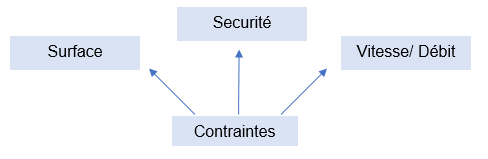
\includegraphics[width=\textwidth]{Cadre_du_Projet/Contraintes.png}
		\caption{Contraintes Principales}
		\label{fig:Contraintes}
	\end{center}
\end{figure}
 
La solution doit aussi respecter des normes internationales de sécurité, particulièrement la ISO 13849-1, qui définit le concept de \textit{Performance Level} auquel l'architecture de contrôle \textit{Dual Check Safety} a été conçu pour suivre.
Les cartons, palettes et préhenseur ont des dimensions déterminées, par contre les dimensions des convoyeurs peuvent être redimensionnés afin d’obtenir une meilleure solution. \par
Ayant ceci en tête, les trois contraintes principales sont la surface de l’îlot de sécurité, la vitesse de palettisation/débit de la cellule et la performance de sécurité. Il est évident qu’on peut réduire la surface si on rapproche la barrière de sécurité près du robot, mais cela rapproche aussi les ouvriers du robot, ce qui peut les mettre en danger.\newpage De façon similaire, si on réduit la vitesse du robot, afin de réduire le risque de chute d’objets, on peut compromettre le flux de production.    



En somme, toute solution proposé doit impérativement:
\begin{itemize}
\item Avoir une surface totale maximum de 6,48 $m^2$;
\item Être capable de palletiser et rendre disponibles dans le local approprié 411 cartons/heure; 
\item Être en accord avec la norme de sécurité ISO 13849-1. 

\end{itemize}
En respectant tous ces critères, nous chercherons minimiser la surface totale, le budget prévu, minimiser les risques de sécurité et maximiser la durée de vie du robot, tout en cherchant une solution réaliste.
Il est très importante d’observer que, basé sur l’avant-projet, nous allons considérer la surface de l’îlot comme la région qui comprend la partie externe de la barrière de sécurité, tandis que l’emplacement où les cartons arrivent sur la cellule et l’emplacement d’où les palettes sont enlevées n’en font pas partie. 